\newpage
\onecolumn
\begin{center}
{\Large{\textbf{Appendix}}}
\end{center}

\begin{appendix}
\section{Neural Path Framework For CNN}\label{sec:cnpf}
\textbf{Indexing:} The weights of layers $l\in[\dc]$ are denoted by $\Theta(\icin,\iin,\iout,l)$ and for layers $l\in[\dfc]+\dc$ are denoted by $\Theta(\iin,\iout,l)$. The pre-activations, gating and hidden unit outputs are denoted by $q_{x,\Theta}(\ifout,\iout,l)$,  $G_{x,\Theta}(\ifout,\iout,l)$, and $z_{x,\Theta}(\ifout,\iout,l)$ for layers $l=1,\ldots, \dc$. $\iin$ and $\iout$ are used to index the input and the output filters. $\ifout$ is used to denote the index of hidden unit (in the feature dimension) within the input and output filters. %Here, $\icin\in[\wconv]$, for $l=1\ldots,\dc$, $\iin\in[w]$ for $l=\dc+2,\ldots,\dc+\dfc+1$, $\ifin \in[1]$ for $l=1$, $\ifin \in[w]$ for $l=2,\ldots,\dc$, $\iout\in[w]$ for $l=1\ldots,\dc, \dc+2,\ldots, \dc+\dfc$,  $\iout\in[1]$ for $l=\dc+\dfc+1$, $\ifout\in[w]$ for $l=1,\ldots,\dc$.
\begin{comment}
\FloatBarrier
\begin{table}[h]
\centering
\begin{tabular}{|c|ll|}\hline
Index & Range&\\\hline
\multirow{2}{*}{$\iin$} & $\in[\din]$ & for $l=1\ldots,\dc$\\ \cline{2-3}
&$\in[w]$ & for $l=\dc+2,\ldots,\dc+\dfc+1$\\ \hline
\multirow{2}{*}{$\ifin$} & $\in[1]$ & for $l=1$\\ \cline{2-3}
&$\in[w]$ &for $l=2,\ldots,\dc$\\ \hline
\multirow{2}{*}{$\iout$} & $\in[w]$ &for $l=1\ldots,\dc, \dc+2,\ldots, \dc+\dfc$\\ \cline{2-3}
&$\in[1]$ &for $l=\dc+\dfc+1$\\ \hline
{$\ifout$} & $\in[w]$ &for $l=1,\ldots,\dc$\\ \hline
\end{tabular}
\end{table}
\end{comment}

\textbf{Shapes:} \Cref{fig:shape-main} shows the shapes of the tensors in the convolutional layers of a $1$-dimensional circular CNN considered in this paper. Here, the input is a $1$-dimensional tensor given by $x\in\R^{\din}$. The hidden nodes in a given convolutional layer have a $2$-dimensional shape of $\din\times w$, where $w$ is the number of filters in the layer. The weights of a given convolutional layer have $3$-dimensional shape of $\wconv\times w\times w$,  where $w\times w$ is because of the number of input filters times the number of output filters.
\FloatBarrier
\begin{figure}[h]
\centering
%\resizebox{\columnwidth}{!}{
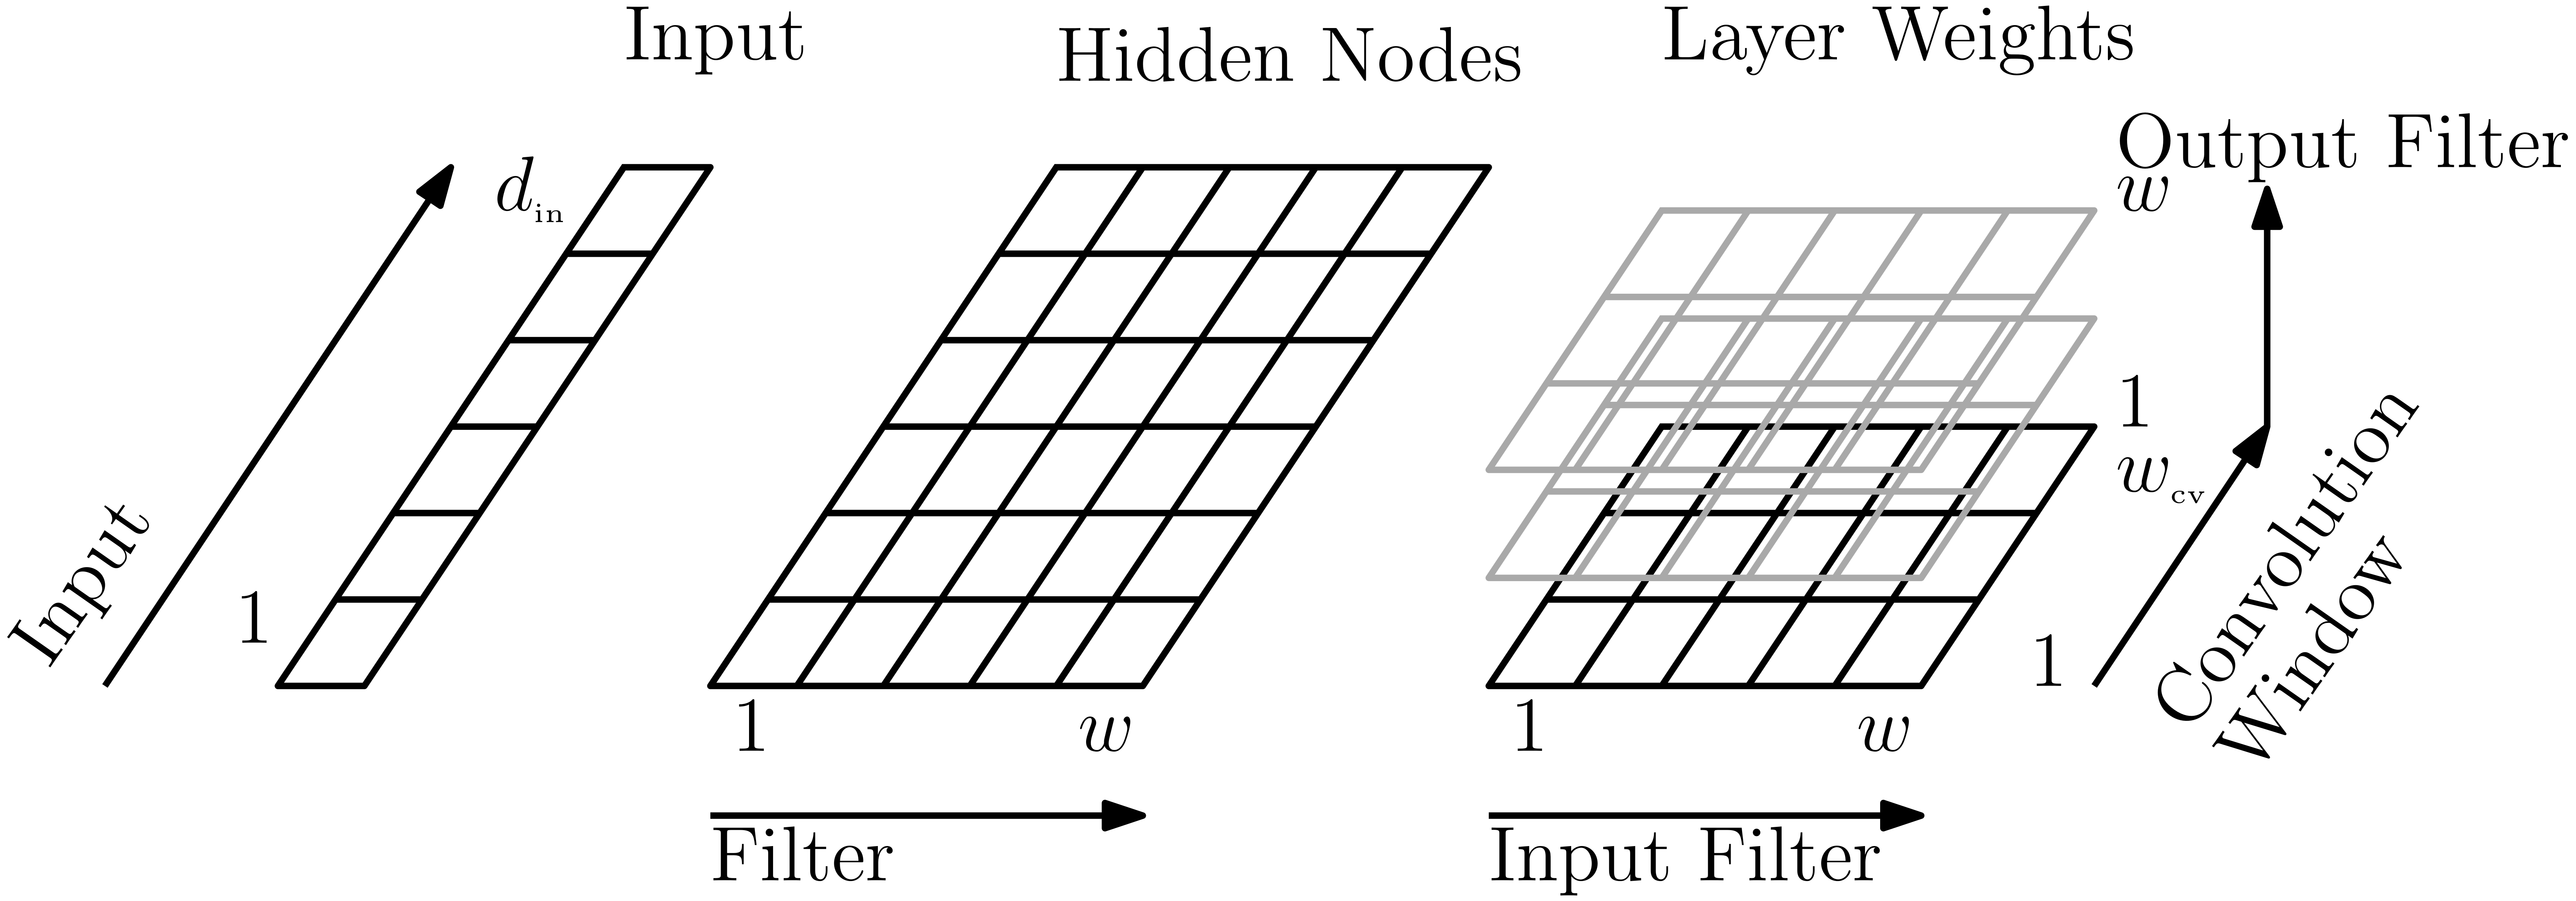
\includegraphics[scale=0.04]{figs/shape.png}
%}
\label{fig:shape-main}
\caption{Shows the shape of the tensor.}
\end{figure}

\subsubsection{Information Flow}
\begin{table}[h]
\centering
\begin{tabular}{|c l lll|}\hline
IL&: &$z_{x,\Theta}(\cdot,1,0)$ &$=$ &$x$ \\\hline\hline
\multicolumn{5}{|l|}{Convolutional Layers, $l\in[\dc]$}\\\hline\hline
PA&: & $q_{x,\Theta}(\ifout,\iout,l)$& $=$ & $\sum_{\icin,\iin}\Theta(\icin,\iin,\iout,l)\cdot z_{x,\Theta}(\ifout\oplus (\icin-1),\iin,l-1)$\\
GV&: &$G_{x,\Theta}(\ifout,\iout,l)$& $=$ & $\mathbf{1}_{\{q_{x,\Theta}(\ifout,\iout,l)>0\}}$\\
HUO&: &$z_{x,\Theta}(\ifout,\iout,l)$ & $=$ & $q_{x,\Theta}(\ifout,\iout,l)\cdot G_{x,\Theta}(\ifout,\iout,l)$\\\hline\hline
\multicolumn{5}{|l|}{GAP Layers, $l=\dc+1$}\\\hline\hline
%HUO&: &${z}_{x,\Theta}(\iout,l)$ & $=$ & $\frac{1}{\din}\sum_{i\in [\din]} z_{x,\Theta}(i,\iout,l-1)$\\\hline\hline
HUO&: &$z_{x,\Theta}(\iout, \dc+1)$ & $=$ &$\sum_{\ifout} z_{x,\Theta}(\ifout,\iout,\dc)\cdot G^{\text{pool}}_{x,\Theta}(\ifout,\iout,\dc+1)$\\\hline\hline
\multicolumn{5}{|l|}{Fully Connected Layers, $l\in[\dfc]+(\dc+1)$}\\\hline\hline
PA&: & $q_{x,\Theta}(\iout,l)$& $=$ & $\sum_{\iin}\Theta(\iin,\iout,l) \cdot z_{x,\Theta}(\iin,l-1) $\\
GV&: &$G_{x,\Theta}(\iout,l)$& $=$ & $\mathbf{1}_{\{(q_{x,\Theta}(\iout,l))>0\}}$\\
HUO&: &$z_{x,\Theta}(\iout,l)$ & $=$ & $q_{x,\Theta}(\iout,l)\cdot G_{x,\Theta}(\iout,l)$\\
FO&: & $\hat{y}_{\Theta}(x)$ & $=$ & $\sum_{\iin}\Theta(\iin,\iout, d)\cdot z_{x,\Theta}(\iin,d-1)$\\\hline
\end{tabular}
\caption{Here IL, PA, GV, HUO, GL and FO are abbreviations for input layer, pre-activation, gating values, hidden unit output, GAP-layer and final output respectively.}
\label{tb:cconv}
\end{table}

\FloatBarrier
\begin{figure}[H]
\centering
\resizebox{\columnwidth}{!}{
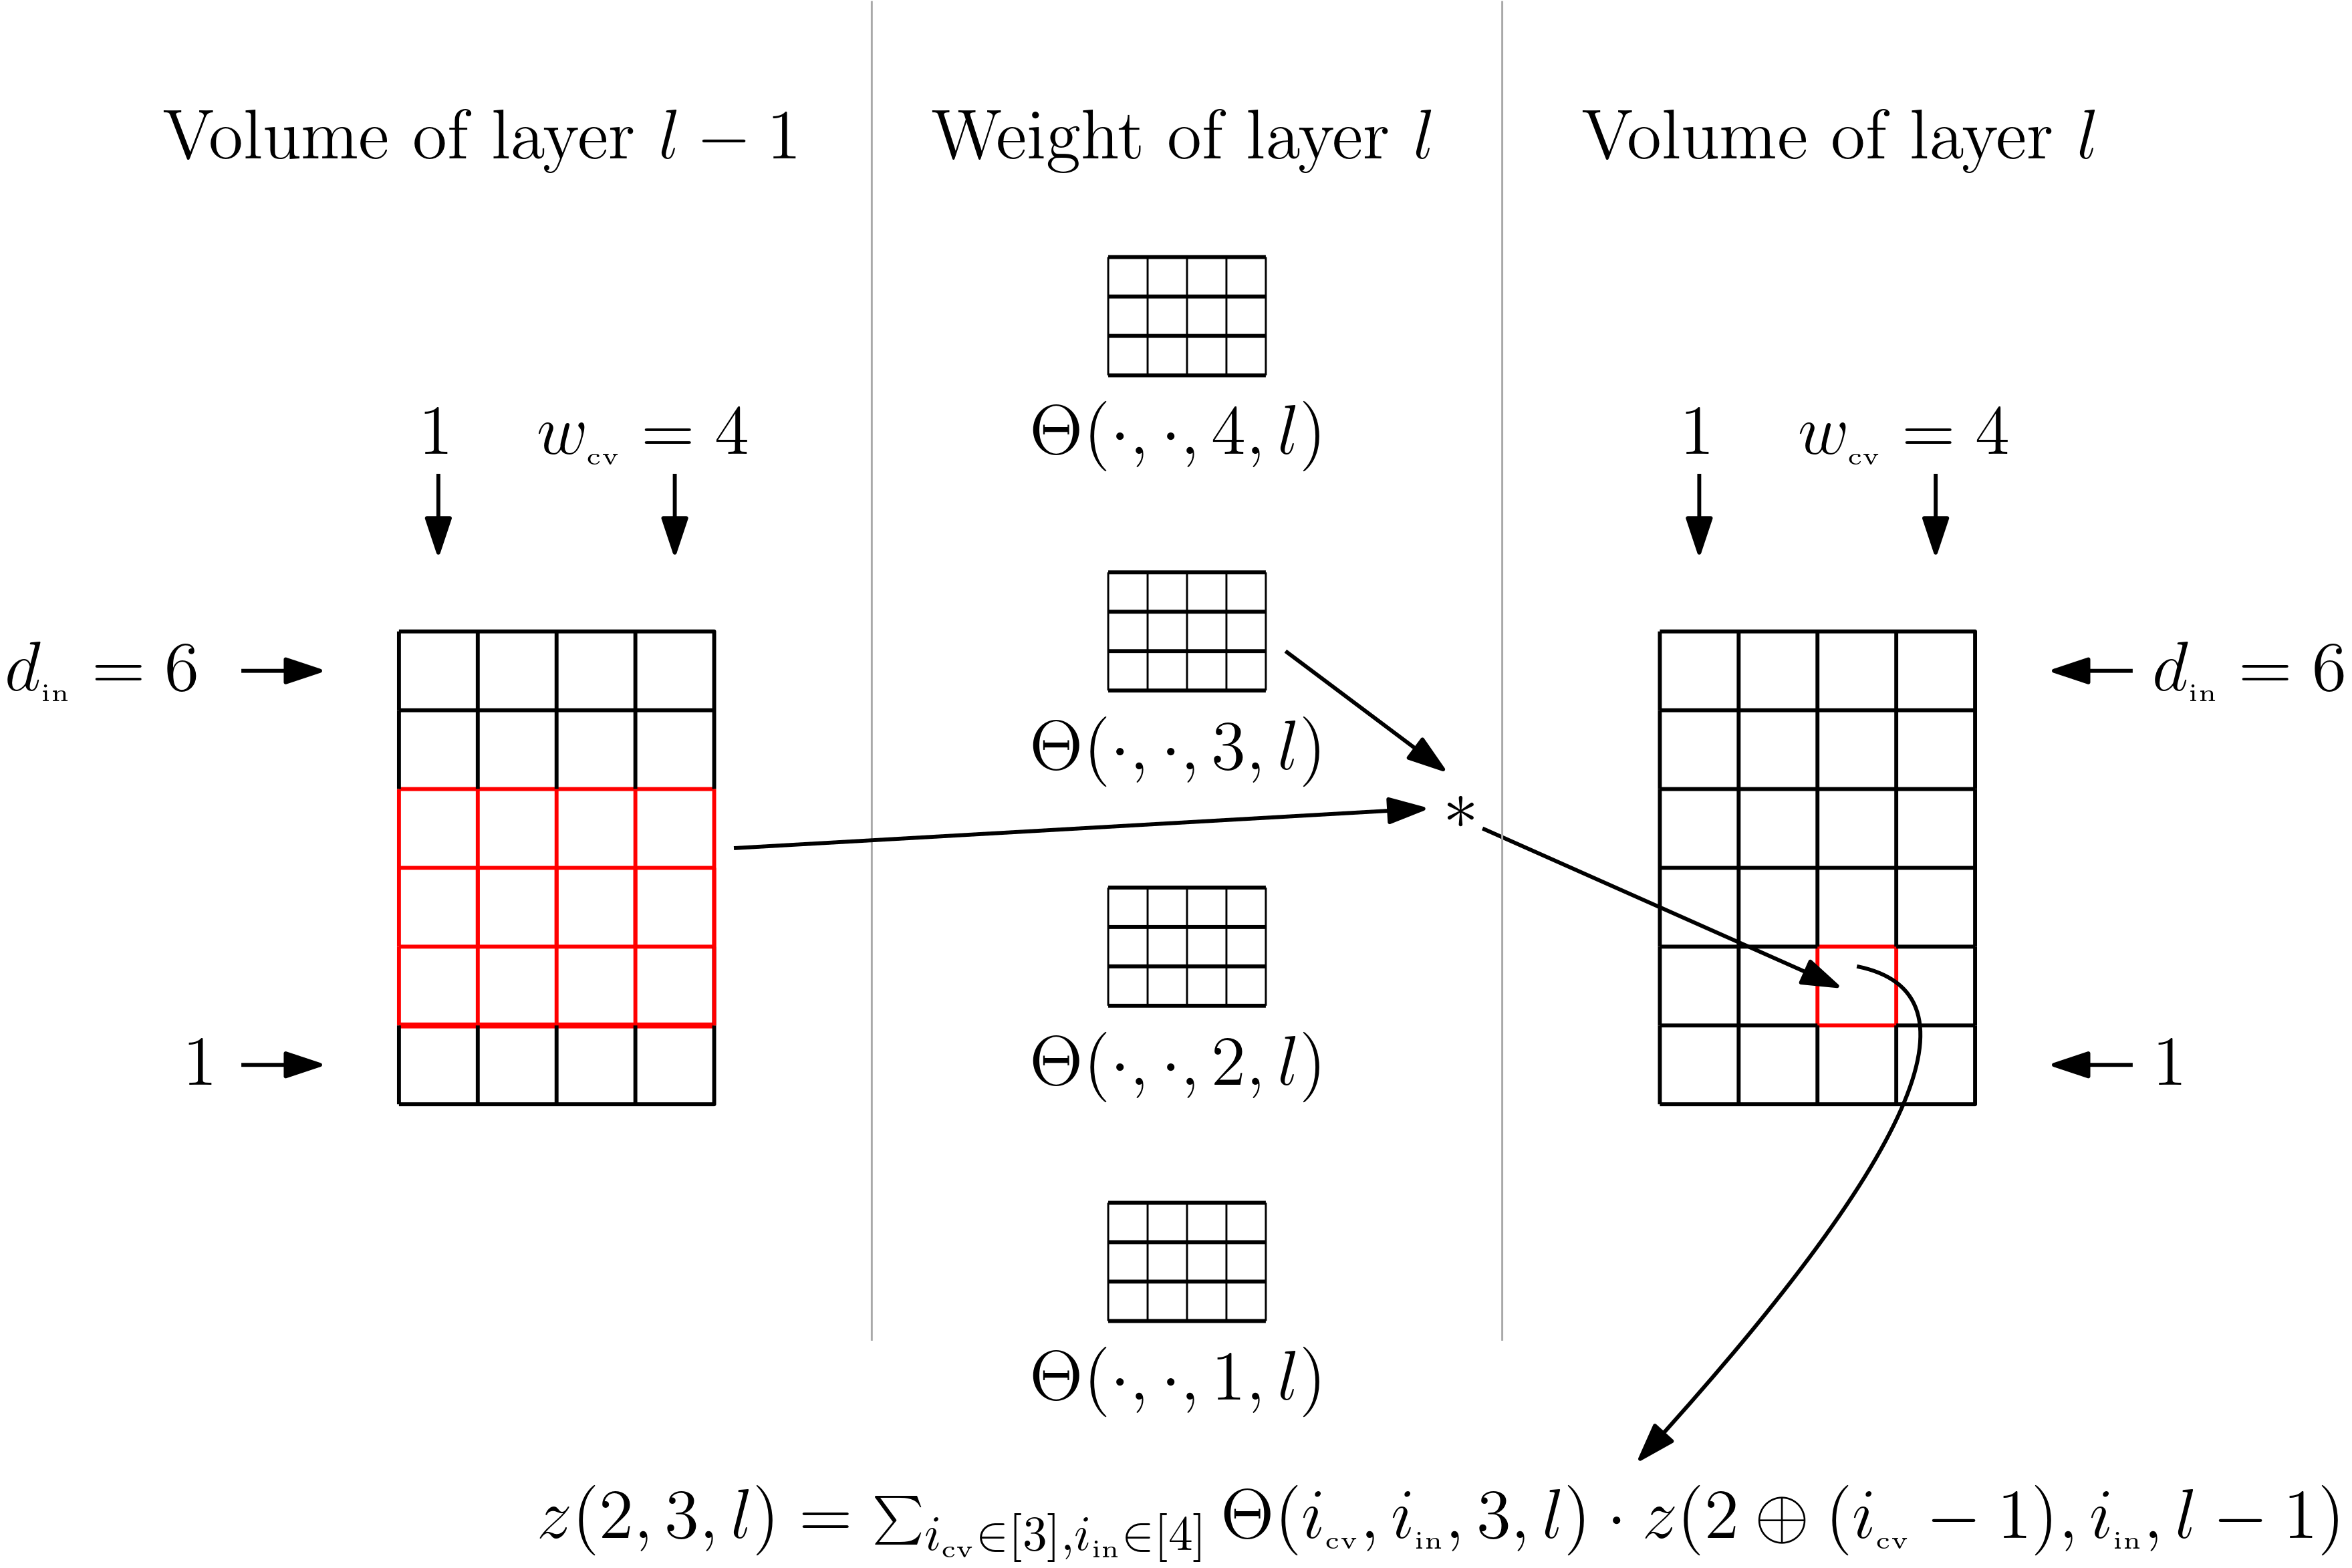
\includegraphics[scale=1]{figs/single-filter.png}
}
\end{figure}
\newpage

\section{Proofs of technical results}

Proof of \Cref{prop:bundle}
\begin{proof}
Note that the total number of paths is $P=\din\cdot (\wconv\cdot w)^{\dc} \cdot \wfc^{(\dfc-1)}$, and in the definition of NPV for CNNs in \Cref{def:bundle} the indices are over only the weights without specifying the input node given by $\Ifeat_{0}(p)$.
\end{proof}

\begin{proposition}[Rotational Invariance]\label{prop:rot}
Internal variables in the convolutional layers are circularly symmetric,  i.e., for $r\in\{0,\ldots,\din-1\}$ it follows that (i) $z_{rot(x,r),\Theta}(\ifout,\cdot,\cdot) = z_{x,\Theta}(\ifout \oplus r,\cdot,\cdot)$, (ii) $q_{rot(x,r),\Theta}(\ifout,\cdot,\cdot) = q_{x,\Theta}(\ifout \oplus r,\cdot,\cdot)$ and (iii) $G_{rot(x,r),\Theta}(\ifout,\cdot,\cdot) = G_{x,\Theta}(\ifout \oplus r,\cdot,\cdot)$.
\end{proposition}


\begin{proof}
For $l=0$, we have $z_{rot(x,r),\Theta}(\ifout, 1, 0) = rot(x,r)(\ifout)= x(\ifout\oplus r) = z_{x,\Theta}(\ifout\oplus r, 1,0)$. Now for $l=1$, we have
\begin{align*}
q_{rot(x,r),\Theta}(\ifout,\cdot,1) &= \sum_{\iin\in[1],\icin\in[\wconv]}\Theta(\icin,\iin,\iout,l)\cdot z_{rot(x,r),\Theta}(\ifout \oplus(\icin-1),\iin,0)\\
&= \sum_{\iin\in[1],\icin\in[\wconv]}\Theta(\icin,\iin,\iout,l)\cdot z_{x,\Theta}((\ifout\oplus r) \oplus (\icin-1),\iin,0)\\
&= q_{x,\Theta}(\ifout\oplus r,\cdot,1) 
\end{align*}
The proof follows by noting that $G=\mathbf{1}_{\{q>0\}}$, and $z=q\cdot G$, and repeating the above argument for the layer $l=2,\ldots, \dc$.
\end{proof}


Proof of \Cref{lm:sumofproduct}
\begin{proof}
\begin{align}
\ip{\phi_{x_s,\Theta},\phi_{x_{s'},\Theta}}&=\sum_{p\in[P]}x_s(\I_0(p))x_{s'}(\I_0(p))A_{\Theta}(x_s,p)A_{\Theta}(x_{s'},p)\nn\\
&=\sum_{i=1}^{\din}x_s(i)x_{s'}(i)\Lambda_{\Theta}(i,x_s,x_{s'})\nn\\
&=\ip{x_s,x_{s'}}_{\Lambda_{\Theta}(\cdot,x_s,x_{s'})}
\end{align}
Owing to the symmetry in a fully connected network, we have $\Lambda(i,x_s,x_{s'})$ to be the same for all values of $i\in[\din]$. And since $H^{\text{lyr}}_{l,\Theta}(s,s')$ measure the number of gates in layer `$l$' that are active for both inputs $x_s$ and $x_{s'}$, the total number of paths active for both inputs is $\Pi_{l=1}^{(d-1)} H^{\text{lyr}}_{l,\Theta}(s,s')$.
\end{proof}

Proof of \Cref{lm:sumofproduct}
\begin{proof}
Proof is complete by noting that the NPF of the ResNet is a concatenation of the NPFs of the $2^b$ distinct sub-FC-DNNs within the ResNet architecture.
\end{proof}


Proof of \Cref{lm:cnnnpk}
\begin{proof}
For the CNN architecture considered in this paper, each bundle has exactly $\din$ number of paths, each one corresponding to a distinct input node. For a bundle $b_{\hat{p}}$, let $b_{\hat{p}}(i),i\in[\din]$ denote the path starting from input node $i$.
\begin{align*}
&\sum_{\hat{p}\in [\hat{P}]} \Bigg(\sum_{i,i'\in[\din]} x(i) x'(i') A_{\Theta}\left(x,b_{\hat{p}}(i)\right) A_{\Theta}\left(x',b_{\hat{p}}(i')\right) \Bigg)\\
=&\sum_{\hat{p}\in [\hat{P}]}\Bigg(\sum_{i\in[\din],i'=i\oplus r, r\in\{0,\ldots,\din-1\}} x(i) x'(i\oplus r) A_{\Theta}\left(x,b_{\hat{p}}(i)\right) A_{\Theta}\left(x',b_{\hat{p}}(i\oplus r)\right)\Bigg)\\
=&\sum_{\hat{p}\in [\hat{P}]}\Bigg(\sum_{i\in[\din], r\in\{0,\ldots,\din-1\}} x(i) rot(x',r)(i) A_{\Theta}\left(x,b_{\hat{p}}(i)\right) A_{\Theta}\left(rot(x',r),b_{\hat{p}}(i)\right)\Bigg)\\
=&\sum_{r=0}^{\din-1} \Bigg(\sum_{i\in[\din]} x(i) rot(x',r)(i) \sum_{\hat{p}\in [\hat{P}]}  A_{\Theta}\left(x,b_{\hat{p}}(i)\right) A_{\Theta}\left(rot(x',r),b_{\hat{p}}(i)\right)\Bigg)\\
=&\sum_{r=0}^{\din-1}\Bigg(\sum_{i\in[\din]} x(i) rot(x',r)(i) \Lambda_{\Theta}(i,x,rot(x',r))\Bigg)\\
=&\sum_{r=0}^{\din-1} \ip{x,rot(x',r)}_{\Lambda_{\Theta}(\cdot,x,rot(x',r))}
\end{align*}
\end{proof}

Proof of \Cref{th:main} follows in the same manner as the proof Theorem~$5.1$ of \citeauthor{ch2020neural} (2020).

\begin{comment}
\begin{lemma}\label{lm:dot}
Let $\varphi_{p,\Theta}$ be as in \Cref{def:npvgrad}, under Assumption~\ref{assmp:main}, for paths $p,p_1,p_2\in \P, p_1\neq p_2$, at initialisation we have (i) $\E{\ip{\varphi_{p_1,\Tv_0}, \varphi_{p_2,\Tv_0}}}= 0$, (ii) ${\ip{\varphi_{p,\Tv_0}, \varphi_{p,\Tv_0}}}= d\sigma^{2(d-1)}$.
\end{lemma}

\begin{proof}
\begin{align*}
\ip{\varphi_{p_1,\Tv_0}, \varphi_{p_2,\Tv_0}}= \sum_{\tv\in \Tv} \partial_{\tv}v_{\Tv_0}(p_1) \partial_{\tv}v_{\Tv_0}(p_2)
\end{align*}
Let $p\rsa(\cdot)$ denote the fact that path $p$ passes through $(\cdot)$, and let $p\bcancel\rsa(\cdot)$ denote the fact that path $p$ does not pass through $\bcancel\rsa$. Let $\tv\in\Tv$ be any weight such that $p\rsa \tv$, and w.l.o.g let $\tv$ belong to layer $l'\in[d]$. If either $p_1\bcancel{\rsa}\tv$ or $p_2\bcancel{\rsa}\tv$, then it follows that $\partial_{\tv} v_{\Tv_0}(p_1) \partial_{\tv} v_{\Tv_0}(p_2)=0$. In the case when $p_1,p_2\rsa\tv$, we have
\begin{align*}
&\E{\partial_{\tv}v_{\Tv_0}(p_1)\partial_{\tv}v_{\Tv_0}(p_2)}\\
&=\E{\underset{l\neq l'}{\underset{l=1}{\overset{d}{\Pi}}} \Bigg(\Tv_0(l, \I_{l-1}(p_1),\I_{l} (p_1))\Tv_0(l,\I_{l-1} (p_2),\I_{l}(p_2)) \Bigg)}\\
&=\underset{l\neq l'}{\underset{l=1}{\overset{d}{\Pi}}}\E{\Tv_0(l,\I_{l-1}(p_1),\I_{l}(p_1))\Tv_0(l,\I_{l-1}(p_2),\I_{l}(p_2))}
\end{align*}
where the $\E{\cdot}$ moved inside the product because at initialisation the weights (of different layers) are independent of each other.
Since $p_1\neq p_2$, in one of the layers $\tilde{l}\in[d-1],\tilde{l}\neq l'$ they do not pass through the same weight, i.e., $\Tv_0(\tilde{l},\I_{\tilde{l}-1}(p_1),\I_{\tilde{l}}(p_1))$ and $\Tv_0(\tilde{l},\I_{\tilde{l}-1}(p_2),\I_{\tilde{l}}(p_2))$ are distinct weights. Using this fact
\begin{align*}
&\E{\partial_{\tv}v_{\Tv_0}(p_1)\partial_{\tv}v_{\Tv_0}(p_2)}\\
&=\underset{l\neq l',\tilde{l}}{\underset{l=1}{\overset{d}{\Pi}}}\E{\Tv_0(l, \I_{l-1}(p_1),\I_l(p_1))\Tv_0(l,\I_{l-1}(p_2),\I_{l}(p_2))}\\
&=\E{\Tv_0(\tilde{l},\I_{\tilde{l}-1} (p_1),\I_{\tilde{l}}(p_1))}\E{\Tv_0(\tilde{l},\I_{\tilde{l}-1 }(p_2),\I_{\tilde{l}}(p_2))}\\
&=0
\end{align*}

The proof of (ii) is complete by noting that $\sum_{\tv\in\Tv} \partial_{\tv}v_{\Tv_0}(p) \partial_{\tv}v_{\Tv_0}(p)$ has $d$ non-zero terms for a single path $p$ and at initialisation we have 
\begin{align*}
&\partial_{\tv}v_{\Tv_0}(p) \partial_{\tv}v_{\Tv_0}(p) \\
&={\underset{l\neq l'}{\underset{l=1}{\overset{d}{\Pi}}} {\Tv_0}^2(l,\I_{l-1}(p),\I_{l}(p))}\\
&=\sigma^{2(d-1)}
\end{align*}
\end{proof}

\textbf{Detailed version of \Cref{th:main} with proof.}
\begin{theorem}\label{th:mainrefined}
Under \Cref{assmp:main}, and $\frac{4d}{w^2}<1$ it follows that
 \begin{align*}
\E{K_{\Tdgn_0}}&=d\cdot\sigma^{2(d-1)} H_{\text{FNPF}}\\
Var\left[K_{\Tdgn_0}(s,s')\right]&\leq O\left(d^2_{in}\sigma^{4(d-1)}\max\{d^2w^{2(d-2)+1}, d^3w^{2(d-2)}\}\right)
\end{align*}
\end{theorem}

\begin{proof}
We have 
\begin{align*}
\E{K_{\Tdgn_0}}&=\E{\Phi^\top_{\text{FNPF}} \V_{\Tv_0} \Phi_{\text{FNPF}}}\\
&=\E{\Phi^\top_{\text{FNPF}} (\nabla_{\Tv}v_{\Tv_0})^\top (\nabla_{\Tv}v_{\Tv_0}) \Phi_{\text{FNPF}}}\\
&=\Phi^\top_{\text{FNPF}} \E{(\nabla_{\Tv}v_{\Tv_0})^\top (\nabla_{\Tv}v_{\Tv_0})}\Phi_{\text{FNPF}}\\
&\stackrel{(a)}=d\cdot\sigma^{2(d-1)} \Phi^\top_{\text{FNPF}}\Phi_{\text{FNPF}}\\
&=d\cdot\sigma^{2(d-1)} H_{\text{FNPF}}
\end{align*}
where, $(a)$ follows from \Cref{lm:dot}.

We now turn to the variance calculation. The idea is that we expand  $Var\left[K_0(s,s')\right]=\E{K_0(s,s')^2} -\E{K_0(s,s')}^2$ and identify the terms which cancel due to subtraction and then bound the rest of the terms.

\textbf{Notation:} In what follows, we let $K_0$ to denote $K_{\Tdgn_0}$ and drop superscript V from $\Tv_0$, and subscript $\Tv_0$ from $v_{\Tv_0}$. Further, we assume that the weights can be enumerated as $\theta(1),\ldots, \theta(d_{net})$. We also denote $p\rsa (\cdot)$ to denote the fact that path $p$ passes through $(\cdot)$ and $p\bcancel{\rsa}(\cdot)$ to denote the fact that path $p$ does not pass through $(\cdot)$. We use a shortcut notation $A(s,p)$ instead of $A(x_s,p)$. In what follows, we let $x\in\R^{\din\times n}$ to be the data matrix.

 Let $\theta(m),m\in[d_{net}]$ belong to layer $l'(m)$, then 
\begin{align}\label{eq:kexpect} 
&\E{K_0(s,s')}\nn\\
&=\sum_{m=1}^{d_{net}}\E{\left(\sum_{p_1 \in[P]}x(\I_0(p_1),s)A_0(s,p_1)\frac{\partial v_0(p_1)}{\partial \theta(m)}\right)\left(\sum_{p_2\in[P]}x(\I_0(p_2),s)A_0(s',p_2)\frac{\partial v_0(p_2)}{\partial \theta(m)}\right)}\nn\\
&=\sum_{m=1}^{d_{net}}\E{\sum_{p_1,p_2\in[P]}x(\I_0(p_1),s)A_0(s,p_1)\frac{\partial v_0(p_1)}{\partial \theta(m)}x(\I_0(p_2),s')A_0(s',p_2)\frac{\partial v_0(p_2)}{\partial \theta(m)}}\nn\\
&\stackrel{(a)}=\sum_{m=1}^{d_{net}}\underset{p_1,p_2\rsa\theta(m)}{\sum_{p_1,p_2\in[P]}}x(\I_0(p_1),s)A_0(s,p_1)x(\I_0(p_2),s')A_0(s',p_2) \mathbb{E}\Bigg[\underset{l\neq l'(m)}{\underset{l=1}{\overset{d-1}{\Pi}}} \Tb_0(l,\I_{l-1}(p_1),\I_{l}(p_1)) \nn\\&\Tb_0(l,\I_{l-1}(p_2),\I_{l}(p_2))\Bigg]\nn\\
&\stackrel{(b)}=\sum_{m=1}^{d_{net}}\underset{p_1,p_2\rsa\theta(m)}{\sum_{p_1,p_2\in[P]}}x(\I_0(p_1),s)A_0(s,p_1)x(\I_0(p_2),s')A_0(s',p_2) \underset{l\neq l'(m)}{\underset{l=1}{\overset{d-1}{\Pi}}} \mathbb{E}\Bigg[ \Tb_0(l,\I_{l-1}(p_1),\I_{l}(p_1))\nn\\
& \Tb_0(l,\I_{l-1}(p_2),\I_{l}(p_2))\Bigg]
\end{align}
where $(a)$ follows from the fact that for $p\bcancel{\rsa}\theta(m)$, $\frac{\partial v_0(p)}{\partial \theta(m)}=0$, and $(b)$ follows from the fact that at initialisation the layer weights are independent of each other. Note that the right hand side of \eqref{eq:kexpect} only terms with $p_1=p_2$ will survive the expectation.

In the following expression in \eqref{eq:kexpectsquare}, note that only terms of the form $p_1=p_2$ and $p_3=p_4$ are non-zero.

\begin{align*}
&\E{K_0(s,s')}^2=\\
&\Bigg(\sum_{m=1}^{d_{net}}\underset{p_1,p_2\rsa\theta(m)}{\sum_{p_1,p_2\in[P]}}x(\I_0(p_1),s)A_0(s,p_1)x(\I_0(p_2),s')A_0(s',p_2) \underset{l\neq l'(m)}{\underset{l=1}{\overset{d-1}{\Pi}}} \mathbb{E}\Big[\Tb_0(l,\I_{l-1}(p_1),\I_{l}(p_1)) &\\ 
&\Tb_0(l,\I_{l-1}(p_2),\I_{l}(p_2))\Big]\Bigg)\times\\
&\Bigg(\sum_{m'=1}^{d_{net}}\underset{p_3,p_4\rsa\theta(m')}{\sum_{p_3,p_4\in[P]}}x(\I_0(p_3),s)A_0(s,p_3)x(\I_0(p_4),s')A_0(s',p_4) \underset{l\neq l'(m')}{\underset{l=1}{\overset{d-1}{\Pi}}} \mathbb{E}\Big[\Tb_0(l,\I_{l-1}(p_3),\I_{l}(p_3)) &\\
&\Tb_0(l,\I_{l-1}(p_4),\I_{l}(p_4))\Big]\Bigg)\\
\end{align*}
\begin{align}\label{eq:kexpectsquare}
&\E{K_0(s,s')}^2=\nn\\
&\sum_{m,m'=1}^{d_{net}}\underset{p_3,p_4\rsa\theta(m')}{\underset{p_1,p_2\rsa\theta(m)}{\sum_{p_1,p_2,p_3,p_4\in[P]}}}\Bigg[\bigg(x(\I_0(p_1),s)A_0(s,p_1)x(\I_0(p_2),s')A_0(s',p_2)x(\I_0(p_3),s)\nn\\ 
&A_0(s,p_3)x(\I_0(p_4),s')A_0(s',p_4)\bigg)\times \bigg( \underset{l\neq l'(m)} {\underset{l\neq l'(m')}{\underset{l=1}{\overset{d-1}{\Pi}}}} \E{\Tb_0(l,\I_{l-1}(p_1),\I_{l}(p_1)) \Tb_0(l,\I_{l-1}(p_2),\I_{l}(p_2))}\nn\\
&\E{\Tb_0(l,\I_{l-1}(p_3),\I_{l}(p_3)) \Tb_0(l,\I_{l-1}(p_4),\I_{l}(p_4))} \bigg)\times\nn\\
&\bigg( \E{\Tb_0(l,\I_{l'(m')-1}(p_1),\I_{l'(m')}(p_1)) \Tb_0(l,\I_{l'(m')-1}(p_2),\I_{l'(m')}(p_2))}\bigg)\times\nn\\
&\bigg(\E{\Tb_0(l,\I_{l'(m)-1}(p_3),\I_{l'(m)}(p_3)) \Tb_0(l,\I_{l'(m)-1}(p_4),\I_{l'(m)}(p_4))} \bigg)\Bigg]
\end{align}
In the expression in \eqref{eq:ksquareexpect}, paths $p_1,p_2,p_3,p_4$ do not have constraints, and can be distinct.
\begin{align}\label{eq:ksquareexpect}
&\E{K^2_0(s,s')}=\nn\\
&\sum_{m,m'=1}^{d_{net}}\underset{p_3,p_4\rsa\theta(m')}{\underset{p_1,p_2\rsa\theta(m)}{\sum_{p_1,p_2,p_3,p_4\in[P]}}}\Bigg[\bigg(x(\I_0(p_1),s)A_0(s,p_1)x(\I_0(p_2),s')A_0(s',p_2)x(\I_0(p_3),s)\nn\\&
A_0(s,p_3)x(\I_0(p_4),s')A_0(s',p_4)\bigg)\times\bigg( \underset{l\neq l'(m)} {\underset{l\neq l'(m')}{\underset{l=1}{\overset{d-1}{\Pi}}}} \mathbb{E}[\Tb_0(l,\I_{l-1}(p_1),\I_{l}(p_1)) \Tb_0(l,\I_{l-1}(p_2),\I_{l}(p_2))\nn\\&
\Tb_0(l,\I_{l-1}(p_3),\I_{l}(p_3)) \Tb_0(l,\I_{l-1}(p_4),\I_{l}(p_4))] \bigg)\times\nn\\
&\bigg( \E{\Tb_0(l,\I_{l'(m')-1}(p_1),\I_{l'(m')}(p_1)) \Tb_0(l,\I_{l'(m')-1}(p_2),\I_{l'(m')}(p_2))}\bigg)\times\nn\\
&\bigg(\E{\Tb_0(l,\I_{l'(m)-1}(p_3),\I_{l'(m)}(p_3)) \Tb_0(l,\I_{l'(m)-1}(p_4),\I_{l'(m)}(p_4))} \bigg)\Bigg]
\end{align}

We now state the following facts/observations.

$\bullet$ \emph{Fact 1:} Any term that survives the expectation (i.e., does not become $0$) and participates in \eqref{eq:ksquareexpect} is of the form $\sigma^{4(d-1)}\big(x(\I_0(p_1),s)A_0(s,p_1)x(\I_0(p_2),s')A_0(s',p_2)x(\I_0(p_3),s)A_0(s,p_3)x(\I_0(p_4),s')A_0(s',p_4)\big)$, where $p_1,p_2,p_3,p_4$ are free variables. Any term that survives the expectation (i.e., does not become $0$) and participates in participates in \eqref{eq:kexpectsquare} is of the form $\sigma^{4(d-1)}\big(x(\I_0(p_1),s)A_0(s,p_1)x(\I_0(p_2),s')A_0(s',p_2)x(\I_0(p_3),s)A_0(s,p_3)x(\I_0(p_4),s')A_0(s',p_4)\big)$, where $p_1=p_2,p_3=p_4$.

$\bullet$ \emph{Fact 2:} The number of paths through a particular weight $\theta(m)$ in one of the middle layers is $\din w^{d-3}$. The number of paths through a particular weight $\theta(m)$ in the first layer is $w^{d-2}$ . The number of paths through a particular weight $\theta(m)$ in the last layer is $\din w^{d-2}$ .


$\bullet$ \emph{Fact 3:} Let $\P'$ be an arbitrary set of paths constrained to pass through some set of weights. Let $\P''$ be the set of paths obtained by adding an additional constraint that the paths also should pass through a particular weight say $\theta(m)$. Now, if $\theta(m)$ belongs to :

$1.$ a middle layer, then $|\P''|=\frac{|\P'|}{w^2}$.

$2.$ the first layer, then $|\P''|=\frac{|\P'|}{\din w}$.

$3.$  the last layer, then $|\P''|=\frac{|\P'|}{w}$.

$\bullet$ \emph{Fact 4:} For any $p_1,p_2,p_3,p_4$ combination that survives the expectation in \eqref{eq:ksquareexpect} can be written as 

\begin{align*}
&\bigg(x(\I_0(p_1),s)A_0(s,p_1)x(\I_0(p_2),s')A_0(s',p_2)x(\I_0(p_3),s)\\
&A_0(s,p_3)x(\I_0(p_4),s')A_0(s',p_4)\bigg)\times\\
&\bigg( \underset{l\neq l'(m)} {\underset{l\neq l'(m')}{\underset{l=1}{\overset{d-1}{\Pi}}}} \mathbb{E}[\Tb_0(l,\I_{l-1}(p_1),\I_{l}(p_1)) \Tb_0(l,\I_{l-1}(p_2),\I_{l}(p_2))\nn\\
&\Tb_0(l,\I_{l-1}(p_3),\I_{l}(p_3)) \Tb_0(l,\I_{l-1}(p_4),\I_{l}(p_4))] \bigg)\times\nn\\
&\bigg( \E{\Tb_0(l,\I_{l'(m')-1}(p_1),\I_{l'(m')}(p_1)) \Tb_0(l,\I_{l'(m')-1}(p_2),\I_{l'(m')}(p_2))}\bigg)\times\nn\\
&\bigg(\E{\Tb_0(l,\I_{l'(m)-1}(p_3),\I_{l'(m)}(p_3)) \Tb_0(l,\I_{l'(m)-1}(p_4),\I_{l'(m)}(p_4))} \bigg)\nn\\
%&=\\
%&\bigg( \underset{l\neq l'(m)} {\underset{l\neq l'(m')}{\underset{l=1}{\overset{d-1}{\Pi}}}} \Tb^2_0(l,\I_{l-1}(\rho_a),\I_{l}(\rho_a)) \Tb^2_0(l,\I_{l-1}(\rho_b),\I_{l}(\rho_b)) \bigg)\times \bigg( \Tb^2_0(l,\I_{l'(m')-1}(\rho_a),\I_{l'(m')}(\rho_a))\bigg)\nn\\
%&\times \bigg({\Tb^2_0(l,\I_{l'(m)-1}(\rho_b),\I_{l'(m)}(\rho_b))} \bigg),
\end{align*}

where $\rho_a\rsa \theta(m)$ and $\rho_b\rsa \theta(m')$ are what we call as \emph{base} (case) paths. 


$\bullet$ \emph{Fact 5:} For any given base paths $\rho_a$ and $\rho_b$ there could be multiple assignments possible for $p_1,p_2,p_3,p_4$.

$\bullet$ \emph{Fact 6:}  Terms in \eqref{eq:ksquareexpect}, wherein, the base case is generated as $p_1=p_2=\rho_a$ and $p_3=p_4=\rho_b$ (or $p_1=p_2=\rho_b$ and $p_3=p_4=\rho_a$), get cancelled with the corresponding terms in \eqref{eq:kexpectsquare}.

$\bullet$ \emph{Fact 7:}  When the bases paths $\rho_a$ and $\rho_b$ do not intersect (i.e., do not pass through the same weight in any one of the layers), the only possible assignment is $p_1=p_2=\rho_a$ and $p_3=p_4=\rho_b$ (or $p_1=p_2=\rho_b$ and $p_3=p_4=\rho_a$), and such terms are common in \eqref{eq:ksquareexpect} and \eqref{eq:kexpectsquare}, and hence do not show up in the variance term.


$\bullet$ \emph{Fact 7:} Let base paths $\rho_a$ and $\rho_b$ intersect/cross at layer $l_1, \ldots, l_k, k \in [d-1]$, and let $\rho_a=(\rho_a(1),\ldots,\rho_a(k+1))$ where $\rho_a(1)$ is a sub-path string from layer $1$ to $l_1$, and $\rho_a(2)$ is the sub-path string from layer $l_1+1$ to $l_2$ and so on, and $\rho_a(k+1)$ is the sub-path string from layer $l_k+1$ to the output node. Then the set of paths that can occur in $\E{K_0(s,s')^2}$ are of the form:
\begin{enumerate}
\item $p_1=p_2=\rho_a, p_3=p_4=\rho_b$ (or $p_1=p_2=\rho_b, p_3=p_4=\rho_a$) which get cancelled in the $\E{K_0(s,s')}^2$ term.
\item $p_1=\rho_a$, $p_3=\rho_b$, $p_2=(\rho_b(1),\rho_a(2),\rho_a(3),\ldots,\rho_a(k+1))$, $p_4=(\rho_a(1),\rho_b(2),\rho_b(3),\ldots,\rho_b(k+1))$, which are obtained by \emph{splicing} the base paths in various combinations. Note that for such spliced paths $p_1\neq p_2$ and $p_3\neq p_4$ and hence do not occur in the expression for $\E{K_0(s,s')}^2$ in \eqref{eq:kexpectsquare}.
\end{enumerate}


$\bullet$ \emph{Fact 8:} For $k$ crossings of the base paths there are $4^{k+1}$ splicings possible, and those many terms are extra in the $\E{K_0(s,s')^2}$ expression in \eqref{eq:ksquareexpect}, when compared to the $\E{K_0(s,s')}^2$ expression in \eqref{eq:kexpectsquare}. 

\textbf{Upper Bound:} We now enumerate various possible crossings of the base paths, and calculate an upper bound for the magnitude of the contribution of `spliced' terms to the variance term using the \emph{Fact 1} to \emph{Fact 8}. In short, we find an upper bound for the those terms that do not get cancelled in the variance calculation. Further, without loss of generality we drop $x(\I_0(p))$ and $A(\cdot,\cdot)$ terms in this upper bound calculation.

\begin{tabular}{|c|c|}\hline
Architecture& Constant \\\hline
FC-DNN&	$\cfc=\din^2 d^2\sigma^{4(d-1)}$\\\hline
CNN& $\ccnn=\din^2 d^2\sigma^{4(d-1)}\wconv$\\\hline
ResNet & $\cres=\din^2\left(\sum_{i=0}^b \binom{b}{i} (i+2) d_{\text{block}}\sigma^{2((i+2) d_{\text{block}}-1)} \right)^2$\\\hline
\end{tabular}
\FloatBarrier
\begin{table}[h]
\begin{tabular}{|c|l|c|c|c|}\hline
Case &Crossing					&FC-DNN 					&CNN 									&ResNet\\\hline
1& $1$ F or $1$ L				&$\frac{2\cdot6^2\cfc}{w}$  		&$\frac{2\cdot6^2\ccnn}{w}$ 			&$\frac{2\cdot6^2\cres}{w}$\\\hline
2& $1$ M					&$\frac{36 d\cfc }{w^2}$  			&$\frac{36 d\ccnn}{w^2}$ 						&$\frac{36 d \cres}{w^2}$\\\hline
3& $1$ F and $1$ L				&$\frac{6^3\cfc}{\din w^2}$  		&$\frac{6^3\ccnn}{\din\wconv w^2}$ 	&$\frac{6^3\cres}{\din w^2}$\\\hline
4& $1$ F or $1$ L and $1$ M		&$\left(\frac{6d}{w^2}\right)\left(\frac{2\cdot6^2\cfc}{w}\right)$ &$\left(\frac{6d}{w^2}\right)\left(\frac{2\cdot6^2\ccnn}{w}\right)$  &$\left(\frac{6d}{w^2}\right)\left(\frac{2\cdot6^2\cres}{w}\right)$\\\hline
5& $2$ M 					&$\left(\frac{6d}{w^2}\right)\left(\frac{36 d\cfc }{w^2}\right)$  			&$\left(\frac{6d}{w^2}\right)\left(\frac{36 d\ccnn}{w^2}\right)$ 						&$\left(\frac{6d}{w^2}\right)\left(\frac{36 d \cres}{w^2}\right)$\\\hline
6& $1$ F or $1$ L and $2$ M		&$\left(\frac{6d}{w^2}\right)^2\left(\frac{2\cdot6^2\cfc}{w}\right)$ &$\left(\frac{6d}{w^2}\right)^2\left(\frac{2\cdot6^2\ccnn}{w}\right)$  &$\left(\frac{6d}{w^2}\right)^2\left(\frac{2\cdot6^2\cres}{w}\right)$\\\hline
7& $1$ F and $1$ L and $1$ M 		&$\left(\frac{6d}{w^2}\right)\left(\frac{6^3\cfc}{\din w^2}\right)$  		&$\left(\frac{6d}{w^2}\right)\left(\frac{6^3\ccnn}{\din \wconv w^2}\right)$ 	&$\left(\frac{6d}{w^2}\right)\left(\frac{6^3\cres}{\din w^2}\right)$\\\hline
8& $3$M 					&$\left(\frac{6d}{w^2}\right)^2\left(\frac{36 d\cfc }{w^2}\right)$  			&$\left(\frac{6d}{w^2}\right)^2\left(\frac{36 d\ccnn}{w^2}\right)$ 						&$\left(\frac{6d}{w^2}\right)^2\left(\frac{36 d \cres}{w^2}\right)$\\\hline
Total & Cases 1+4+6+$\ldots$ &$\frac{\cfc}{w}\left(\frac{\cfc'}{1-6dw^{-2}}\right)$ &$\frac{\ccnn}{w}\left(\frac{\ccnn'}{1-6dw^{-2}}\right)$& $\frac{\cres'}{w}\left(\frac{\cres}{1-6dw^{-2}}\right)$\\\hline
Total & Cases 3+7+$\ldots$ &$\frac{d\cfc}{w^2}\left(\frac{\cfc''}{1-6dw^{-2}}\right)$ &$\frac{d\ccnn}{w^2}\left(\frac{\ccnn''}{1-6dw^{-2}}\right)$& $\frac{d\cres}{w^2}\left(\frac{\cres''}{1-6dw^{-2}}\right)$\\\hline
Total & Cases 2+4+6+$\ldots$ &$\frac{\cfc}{w^2}\left(\frac{\cfc'''}{1-6dw^{-2}}\right)$ &$\frac{\ccnn}{w^2}\left(\frac{\ccnn'''}{1-6dw^{-2}}\right)$& $\frac{\cres}{w^2}\left(\frac{\cres'''}{1-6dw^{-2}}\right)$\\\hline
\end{tabular}
\caption{Here `F', `M' and `L' stand for \emph{first, middle} and \emph{last} layers respectively, where middle layer is any layer that is not the first or the last. $1$ F or $1$ L means, $k=1$ crossing of the base paths either in the first or the last layer. $1$ F and $1$ L means $k=2$ crossings of the base paths one in the first layer and the other in the last layer. Similarly $3$ M means, $k=3$ crossings of the base paths, all in the middle (i.e., intermediate) layers.} 
\end{table}
The cases can be extended in a similar way, increasing the number of crossings.  Now, assuming $\frac{6d}{w^2}<1$, the bounds in the various terms can be lumped together as below:

Putting together we have the variance to be bounded by 
\begin{align*}
\cfc\cdot\max\left\{\cfc^{(1)}\cdot\left(\frac{1}{w}\right),\cfc^{(2)}\cdot\left(\frac{d}{w^2}\right)\right\}, \\
\ccnn\cdot\max\left\{\ccnn^{(1)}\cdot\left(\frac{1}{w}\right),\ccnn^{(2)}\cdot\left(\frac{d}{w^2}\right)\right\}, \\
\cres\cdot\max\left\{\cres^{(1)}\cdot\left(\frac{1}{w}\right),\cres^{(2)}\cdot\left(\frac{d}{w^2}\right)\right\}, 
\end{align*}
respectively for FC-DNN, CNN and ResNet. Here, $\cfc^{(i)},\ccnn^{(i)},\cres^{(i)},i=1,2$ are positive constants.
\end{proof}
\end{comment}
\end{appendix}